\documentclass[conference]{IEEEtran}

\usepackage[noadjust]{cite}
\usepackage{subfig}
\usepackage{balance}
\usepackage{verbatim}
\usepackage{flushend}
\usepackage{hyperref}


% *** GRAPHICS RELATED PACKAGES ***
%
\ifCLASSINFOpdf
  \usepackage[pdftex]{graphicx}
  % declare the path(s) where your graphic files are
  % \graphicspath{{../pdf/}{../jpeg/}}
  % and their extensions so you won't have to specify these with
  % every instance of \includegraphics
  % \DeclareGraphicsExtensions{.pdf,.jpeg,.png}
\else
  % or other class option (dvipsone, dvipdf, if not using dvips). graphicx
  % will default to the driver specified in the system graphics.cfg if no
  % driver is specified.
  % \usepackage[dvips]{graphicx}
  % declare the path(s) where your graphic files are
  % \graphicspath{{../eps/}}
  % and their extensions so you won't have to specify these with
  % every instance of \includegraphics
  % \DeclareGraphicsExtensions{.eps}
\fi

\usepackage{algorithm}
\usepackage[noend]{algorithmic}

\usepackage{multirow}
\usepackage{amsmath}
\usepackage{xcolor}

\renewcommand{\algorithmicrequire}{\textbf{Input:}}
\renewcommand{\algorithmicensure}{\textbf{Output:}}

% correct bad hyphenation here
\hyphenation{op-tical net-works semi-conduc-tor}



\begin{document}

\title{Hot Deployment with Dependency Reconstruction}

\author{\IEEEauthorblockN{Haicheng Li, Chun Cao,  Ping Yu}
\IEEEauthorblockA{State Key Lab for Novel Software Technology, Nanjing University, Nanjing, China\\
Dept. of Computer Science and Technology, Nanjing University, Nanjing, China\\
lhc\_happy@sina.cn, \{caochun, yuping\}@nju.edu.cn}
}

% make the title area
\maketitle


\begin{abstract}
%\boldmath
The hot deployment mechanism is a typical feature of mainstream application servers. 
But current application servers only support hot deployment of standalone applications, which cannot satisfy the requirement of modular applications. 
Failures will occur when some depended modules are updated online, which will result in failure of the whole application platform.
To solve the problem, all the dependent modules must be redeployed in a manual or semi-automatic manner at the cost of increasing overhead after deployment of depended modules.
So a new technology of hot deployment with dependency reconstruction is introduced in order to avoid the unnecessary redeployment.
Dependency management and maintenance is placed in module class loaders, so that the cost of dependency reconstruction will be reduced.
Experiments show that our technology of hot deployment can ensure the correctness of modular applications and operating efficiency of application servers will be highly improved.
\end{abstract}

\begin{IEEEkeywords}
Hot deployment; Dependency reconstruction; Class loading.
\end{IEEEkeywords}


\IEEEpeerreviewmaketitle


\section{Introduction\label{sec:introduction}}

Nowadays application servers\cite{app_server} provide platforms for enterprise applications to be deployed, operated and maintained. They usually contain comprehensive services, such as clustering, security and transaction management, et. al, so that developers can focus on the business logic. As one of those sophisticated services, hot deployment enables the server to put applications into production without restarting the server itself. By hot deployment, the existing application can be upgraded in this fashion as well.

The technology of hot deployment highly improves the efficiency and flexibility of the application servers.
It becomes one of the typical features of mainstream application server products, such as JBoss\cite{jboss} and WebLogic\cite{weblogic}, which play a significant role in the development of enterprise applications. By the philosophy of design of the application servers, the units to be deployed, in packages (or modules) of ear/war/jar, are standalone applications, which means they are closed and self-contained. This implicit assumption does not prohibit the developers to build the applications that spans multiple packages with internal dependencies. Applications in this case can still work as long as the referencing across different deployment units are supported. As a matter of fact, the unit deploying mechanisms built in the application servers like JBoss do make this happen with appropriate class loader designed. Application servers ensure that modules are deployed after the deployment of modules which it depends on. The dependencies are constructed in the context of deployment unit during the first time deployment.

Applications in multiple packages, which are called as \emph{modular applications}, are common when they are developed by different individuals collaboratively or assembled with third-party libraries that are already packed independently. They still works fine on application servers until some portion of the application is about to be hot deployed  with the new versions. As the application server treats the packages as isolated ones, it ignores the existence of potential relationships among the modules. Failures may happen because of the original dependencies between the portion to be hot deployed and the rest of the application are broken and applications are actually down\cite{middleware_reliability}.

To solve the problem, the dependencies need to be reconstructed. Intuitively, this can be done manually. The developer should have the knowledge of dependent configuration among the application modules and be aware the affection scope of the redeployment. Then they can redeploy the dependent ones by hand. However, this requires human intervention can be strenuous and even error-prone, especially for large-scale application. Alternatively, they can also redeploy all the modules for that application. But it is not only unnecessary but also cause the state of unaffected part to be destructed, such as data storage module which is hardly updated. 

In this paper, we introduce a general approach to enable the correct hot deployment respecting the dependencies among modules. The dependencies are constructed with class loaders for the modules and upon the dependent modules can be calculated and their hot deployment can be triggered. In order to update flexibly and efficiently, dependency reconstruction can be done in the class loaders. We can get and manage dependencies from the static module profiles or by dynamic way during hot deployment, so that dependent modules only update their class loaders and they don't need to do anything else except class loading in the process of redeployment. Experiment shows the problem of calling failure can be solved through this technology and the efficiency of application servers is improved.

The rest of this paper is organized as follow. 
Section \ref{sec:background} reviews the hot deployment mechanism and analyzes reasons of failures based on hot deployment mechanism. 
Section \ref{sec:reconstructionAS} describes dependency reconstruction in application servers, which is a common approach to solve dependency lost.
And Section \ref{sec:reconstructionCL} presents a more effective approach of dependency reconstruction in class loaders.
We give the evaluations in Section \ref{sec:evaluation} and Section \ref{sec:relatedwork} is the related work.
Lastly in Section \ref{sec:conclusion}, we conclude this paper and discuss future work.



\section{Background\label{sec:background}}
In this section, the hot deployment mechanism of current application servers are reviewed. We also analyze the cause of the failure in hot deploying the modular applications.

\subsection{Hot Deployment}

Hot deployment built in mainstream application servers enables applications on the servers to be are published, updated or withdrawn without restarting the servers. This feature is based on the class loading mechanism beyond the standard class loaders\cite{standard_cl} in Java system. Conceptually, each module, as an standard alone application, to be deployed has its own class loader instead of sharing one with other modules so that standalone applications in that module can be independently operated. All the effective module class loaders are organized together (in a chain or pool) so that they can find each other and delegate each other to load classes and resources which enables the mutual referring and sharing among the modules. When some module are hot deployed, the corresponding module class loader will be removed and a new one will be created to load the new version of the module. In this way, application servers complete hot deployment of applications\cite{module_cl}.

\begin{figure}[ht]
\centering
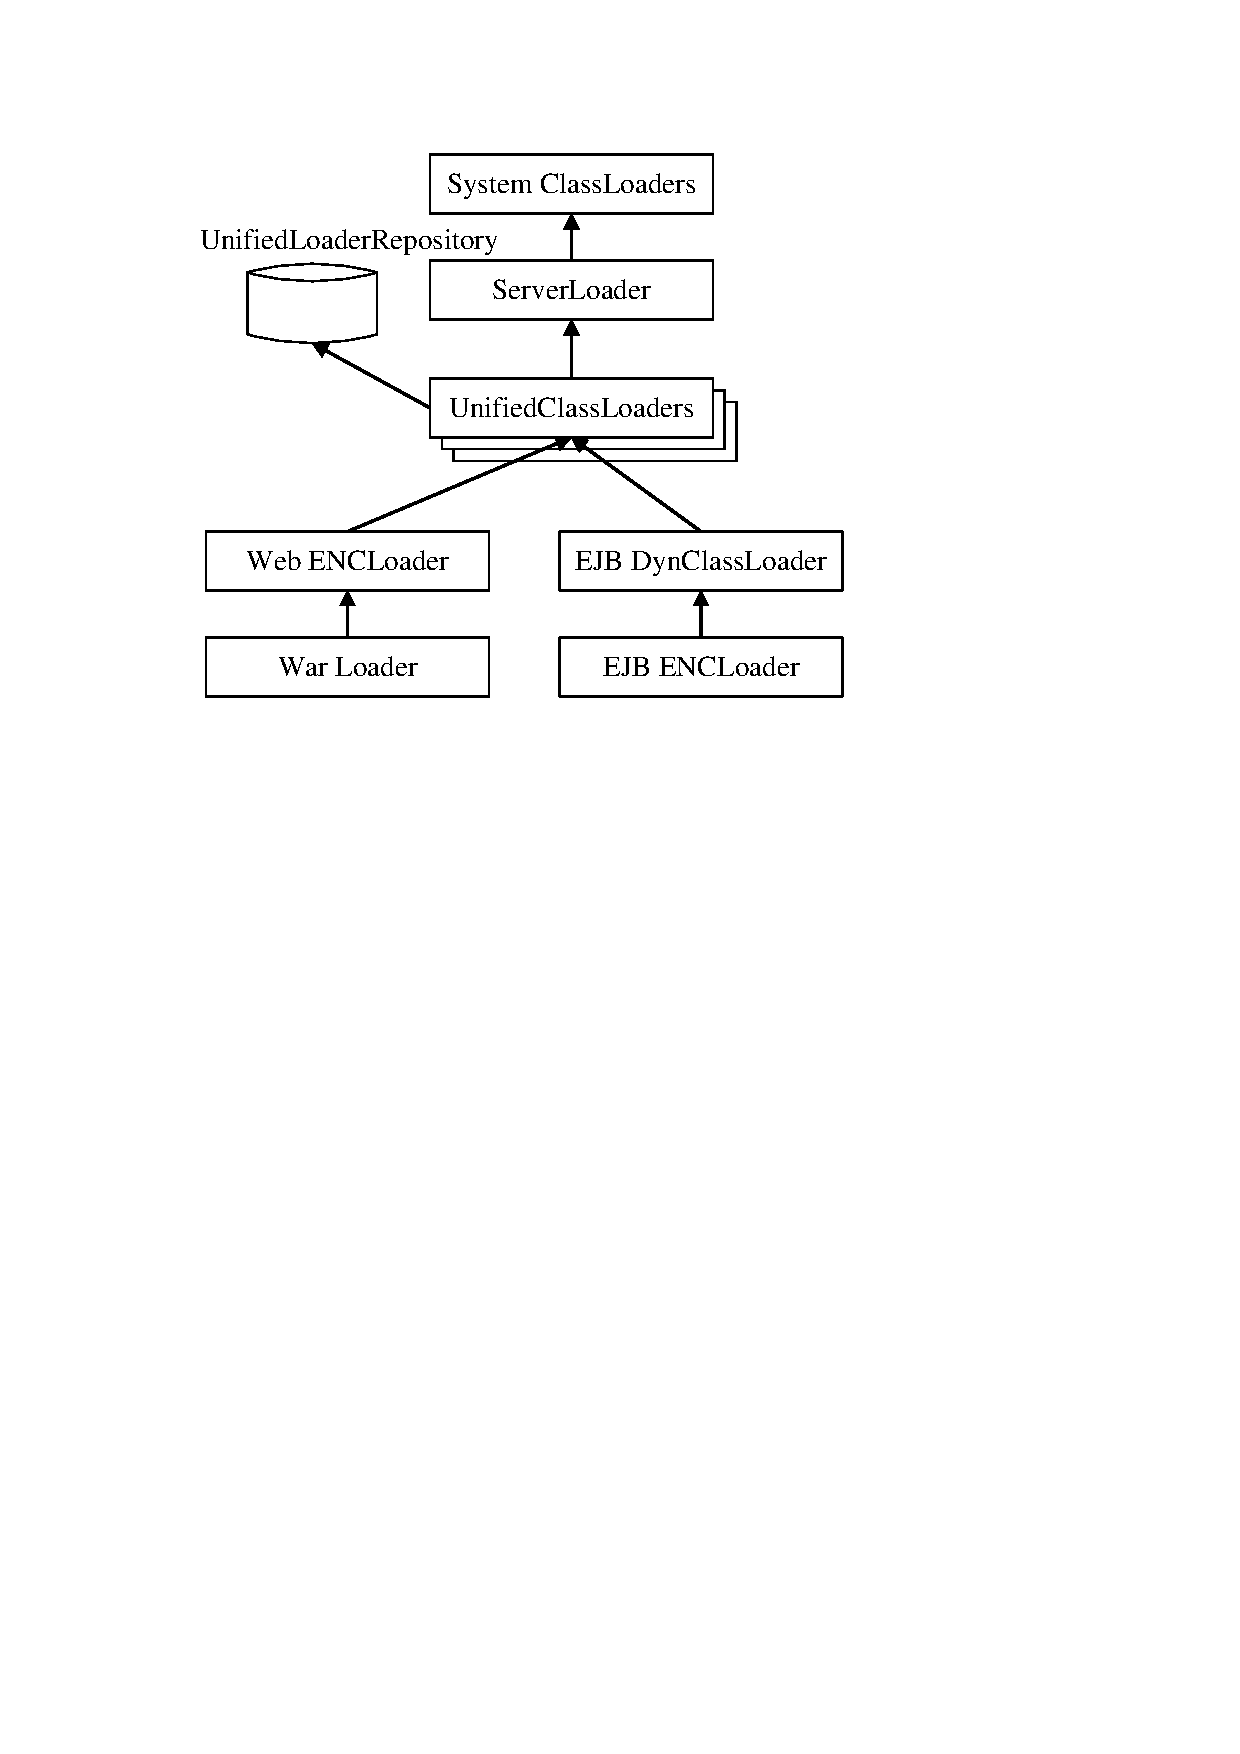
\includegraphics[width=2.5in]{JBossClassLoader.pdf}
\caption{class loader architecture in JBoss}
\label{fig:jboss_class_loader}
\end{figure}

Fig. \ref{fig:jboss_class_loader} shows an illustrative architecture of class loading in JBoss and other application servers adopt similar designs.
As for JBoss, \emph{Sytem ClassLoaders} and \emph{ServerLoader} are responsible to load JBoss server itself. 
The most important class loader is \emph{UnifiedClassLoader}, which covers EARs, JARs, WARs, SARs and directories seen by the deployment scanner as well as JARs referenced by their manifests and any nested deployment units they may contain\cite{jboss_class_loader}. 
For a divison EJB\cite{EJB} application as an example in Fig.\ref{fig:example}, class ComputeBean is a sesion Bean for computing divsion and class ValidatorBean is another session bean to verify the divior is zero or not.
Class ComputeBean is packaged in a module named Compute.jar while class ValidatorBean is packaged in the other module named Validator.jar.
These two modules make up this EJB modular application with dependency injection\cite{DI}.
If this application is deployed in JBoss, \emph{EJB DynClassLoader} and \emph{EJB ENCLoader} are responsible for loading the classes in this EJB applications. Finally, \emph{UnifiedClassLoader} is delegated to load classes and each \emph{UnifiedClassLoader} instance is placed in \emph{UnifiedLoaderRepository} after finishing class loading. Because each \emph{UnifiedClassLoader} instance is responsible for only one module, it is just a module class loader which helps JBoss achieve hot deployment.

\begin{figure}[ht]
\centering
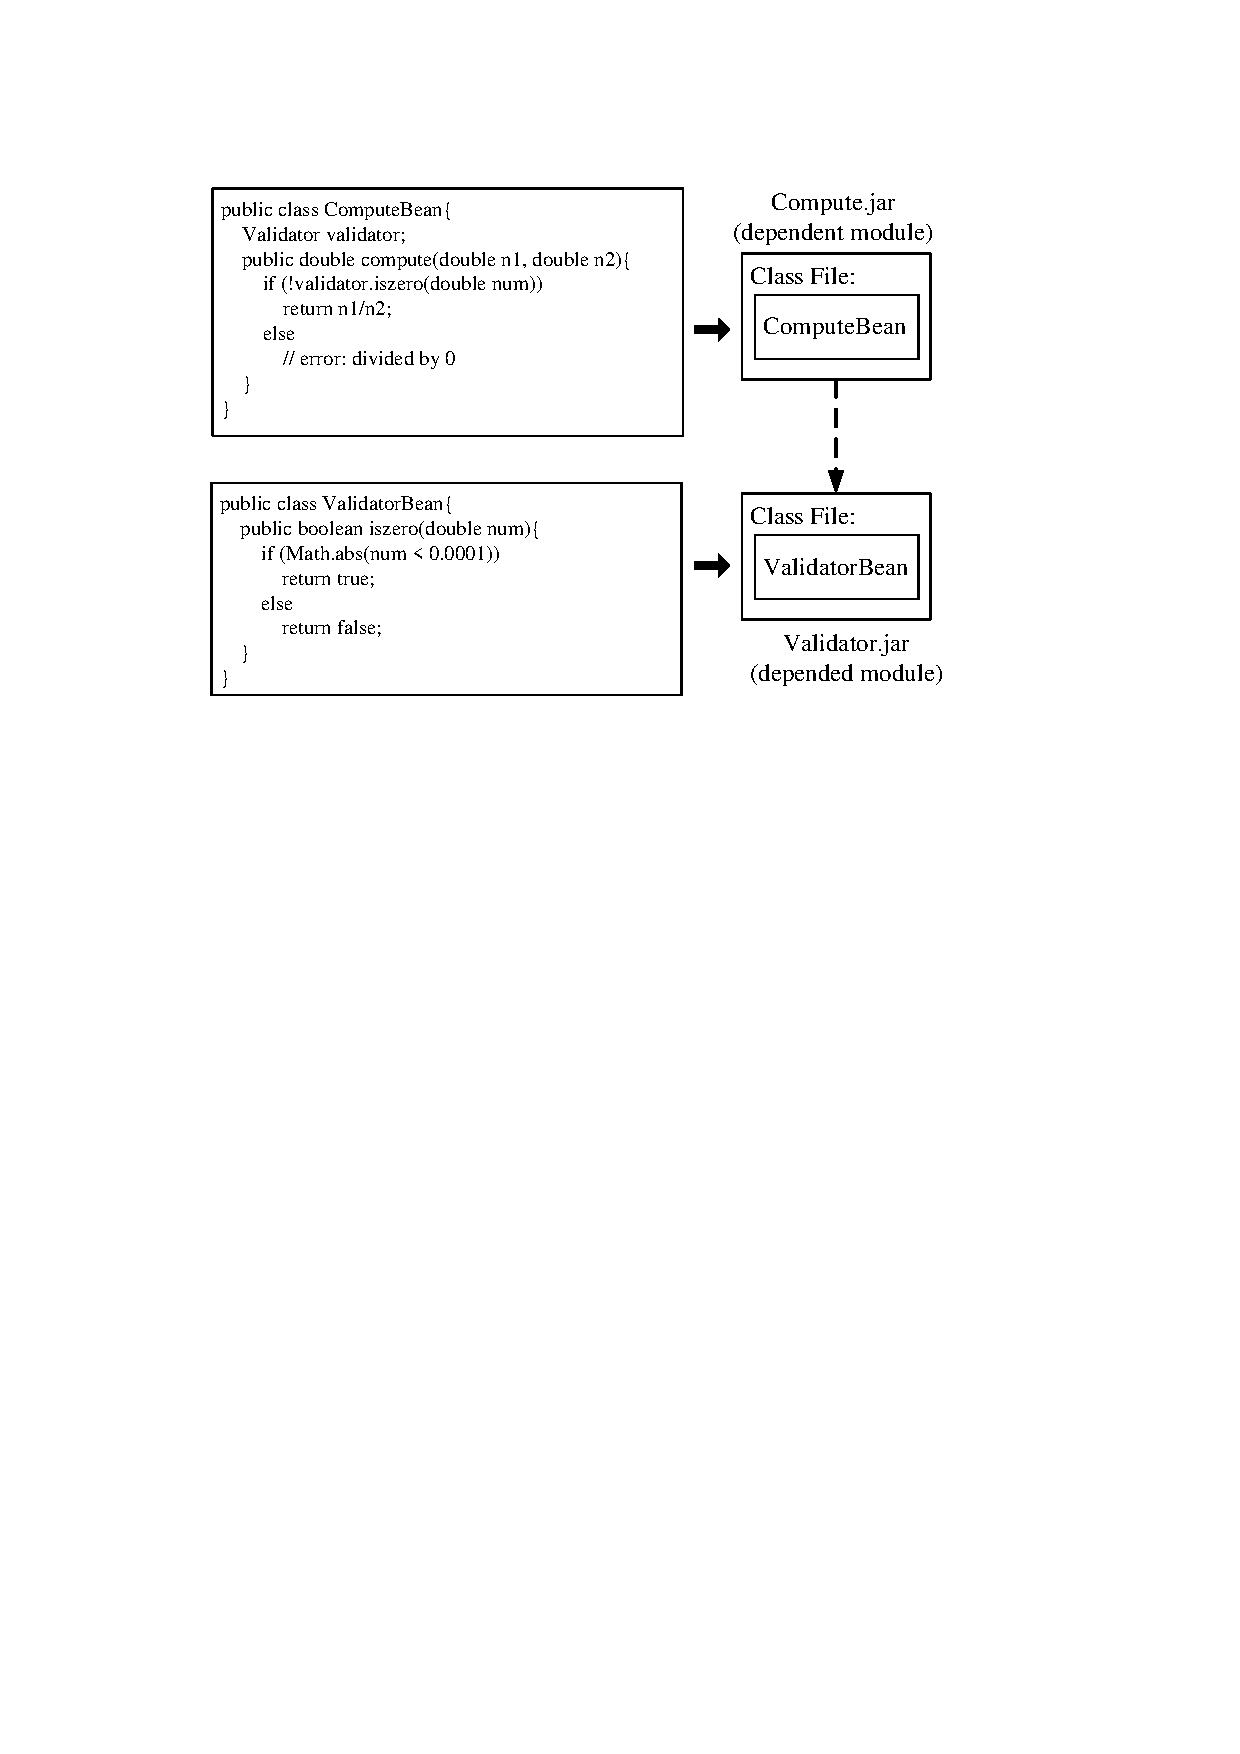
\includegraphics[width=3.5in]{ExampleEJB.pdf}
\caption{a modular application and main source codes}
\label{fig:example}
\end{figure}

%\textcolor{red}{However, most applications are modular applications which are consisted of more than one module containing one or more classes.
%}Fig.\ref{fig:example} is an easy modular application with dependency injection\cite{DI}, which has two EJB\cite{EJB} components deployed in the application server.
From the source codes of two classes in Fig.\ref{fig:example}, the dependency reflects in the divisor must be check whether it is zero when calculating the division of two numbers.
So, in modular applications, a module can be defined as $M=<C, L, R>$. 
$C=\{c_1, c_2, c_3\cdots\}$ is the set of classes in that module. 
$L$ is a module class loader to load all the classes in the class set $C$.
$R=\{M_1, M_2, M_3\cdots\}$ is the set of its dependency against other modules. 
In the division modular application, Compute.jar is a dependent module used to compute division and $R = \{Validator.jar\}$, because class \emph{ComputeBean} calls the method in class \emph{ValidatorBean} and these two classes are in different modules.
Validator.jar is a dependent module used to verify the divisor and $R = \emptyset$, which means Validator.jar doesn’t depends on any modules.


\subsection{Hot Deployment Failures Caused by Module Dependency}

\textcolor{red}{The current application servers have hot deployment capabilities using module class loader architecture.
}\textcolor{red}{If a single module as an application hot deploys, the module class loader will also update with it and application will be running regularly.
However, if a modular application deploys in application servers and only the depended module is hot deployed, hot deployment failures will occur when we execute this modular application.
The reason is that module class loaders load classes from each module separately.
When only a depended module updating online, its original module class loader will be replaced by a new module class loader.
But the module class loader of dependent module still exists, and the module it depends is still an old version which has been removed.
Thus, dependency loss occurs and calling the depended module again will result in call failure.
}

\begin{figure}[ht]
\centering
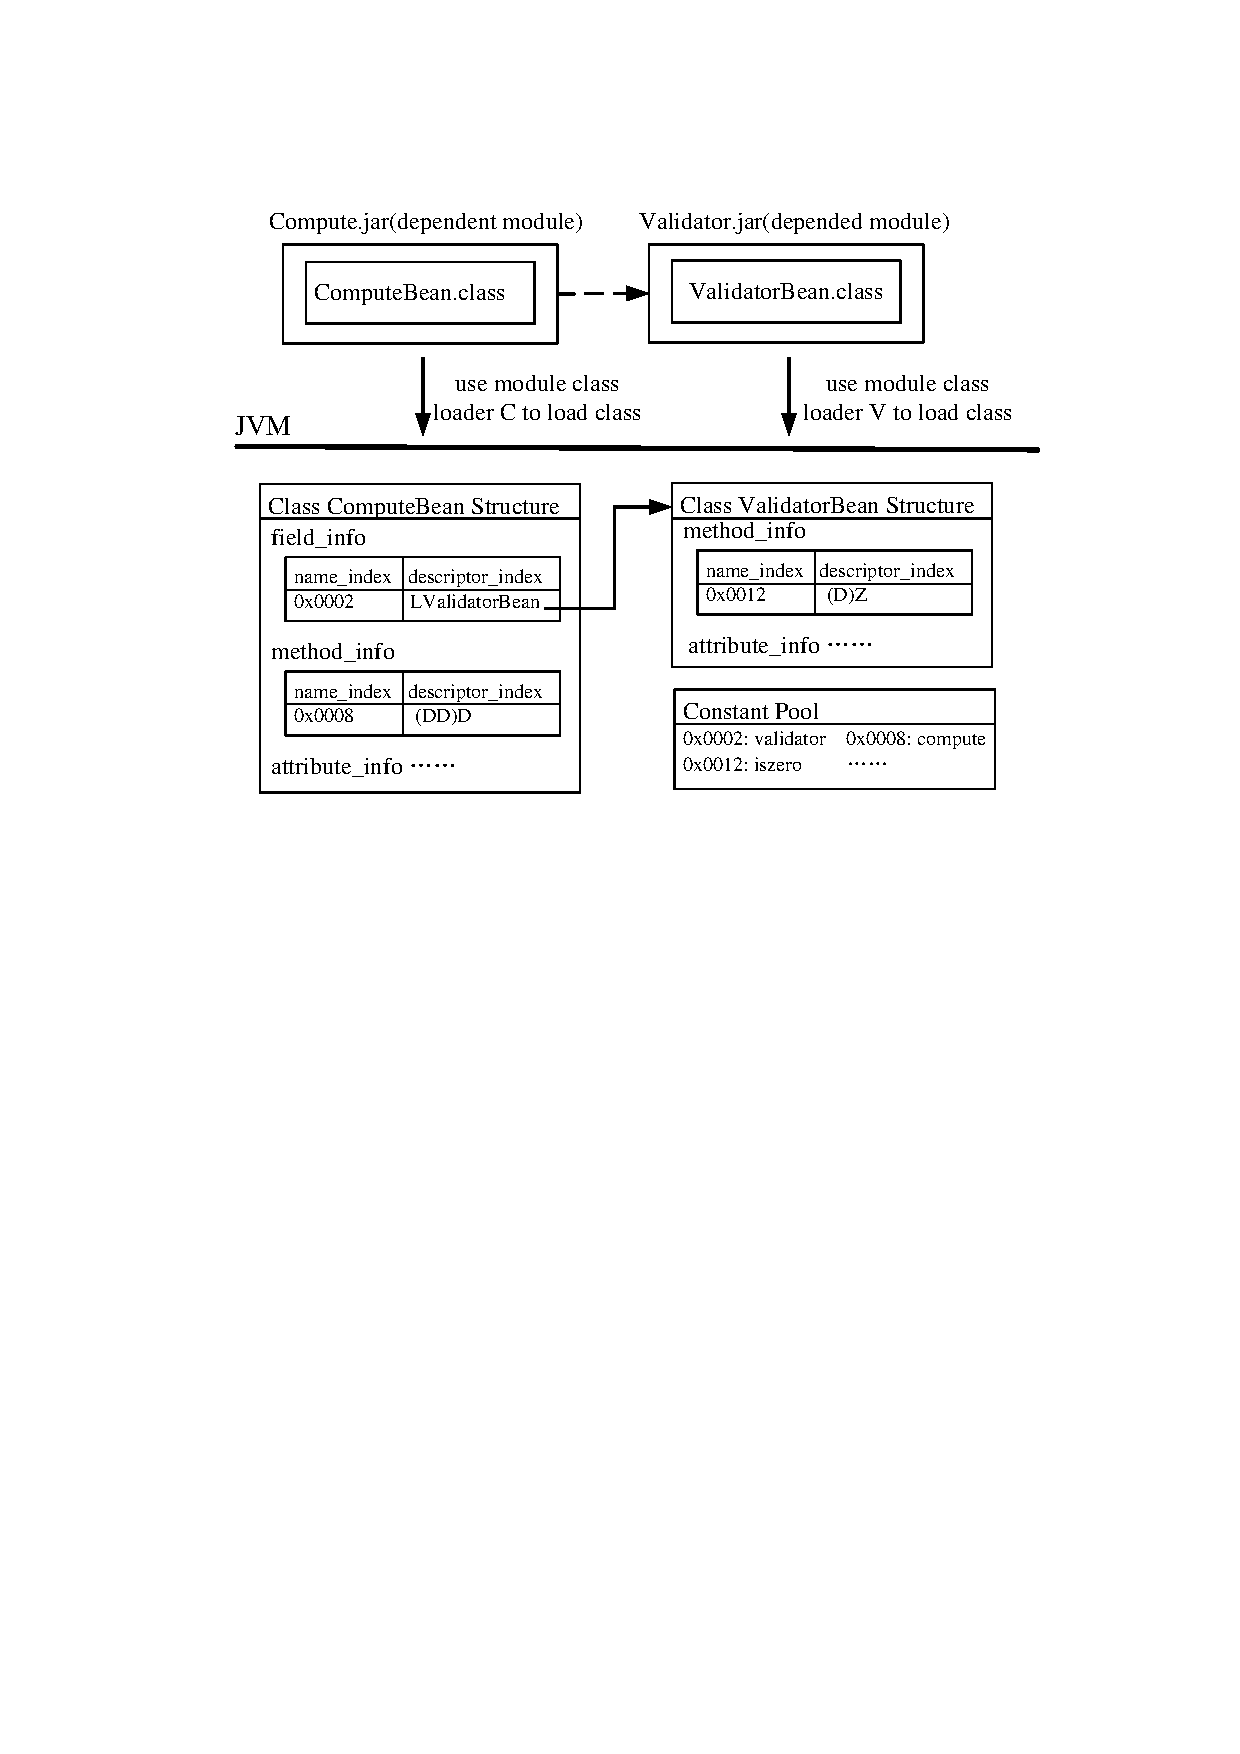
\includegraphics[width=3.5in]{ExampleJVM.pdf}
\caption{a modular application and loading details}
\label{fig:example_jvm}
\end{figure}

For the sample application, when two modules are deployed, the classes in the modules are loaded by module class loaders shown in Fig.\ref{fig:example_jvm}. 
Hot deployment required that each module must have its own class loader instance, so that Class Loader $C$ loads Class \emph{ComputeBean} in Compute.jar while Class Loader $V$ loads Class \emph{ValidatorBean} in Validator.jar.
After class loading, the information of Class \emph{ComputeBean} and Class \emph{ValidatorBean} is resolved and is stored in their own class structure in the Java virtual machine (JVM). 
%JVM is the cornerstone of the Java platforms. It is the component of the technology responsible for its hardware and operating system independence, the small size of its compiled code, and its ability to protect users from malicious programs\cite{jvm}. 
%Here we focus on several class information stored in the class structure. 
Field table which labeled \emph{field\_info} is used to describe the variables declared in the class. 
Method table which labeled \emph{method\_info} is used to describe the methods of the class. 
These two tables have many attributes. 
Some attributes are described in the attribute table labeled \emph{attribute\_info}. 
But our concern is the index marked \emph{name\_index} and \emph{descriptor\_index}. 
In short, we can find the field name \emph{validator} and field type \emph{ValidatorBean} from the index in the \emph{field\_info} of class structure \emph{ComputeBean}. 
The \emph{name\_index} points to the constant pool and the \emph{descriptor\_index} points to the referenced class structure if this variable is a reference type\cite{jvm_book}. 
So, the classes in different modules are associated in the JVM and the JVM can ensure the normal operation of modular applications.

When only the depended module Validator.jar needs to be updated, Validator.jar will be redeployed with the new version of Class \emph{ValidatorBean}. 
The new version of Class \emph{ValidatorBean} may modify some implementation of methods and the modification doesn’t affect implementation of Class \emph{ComputeBean}. 
In this case, Class \emph{ComputeBean} is still the original version and Compute.jar won’t be updated. 
From the JVM specification\cite{jvm_specification}, a class loader cannot load a class twice, which means we cannot use the original Class Loader $V$ to load the new version of Class \emph{ValidatorBean}. 
We should update Class Loader $V$ and use this new class loader to load the new version of Class \emph{ValidatorBean}. 
The class structure of Class \emph{ValidatorBean} in JVM is also updated. 
At this moment, the dependency that JVM creates at the first deployment is lost. 
The index of original class structure of Class \emph{ComputeBean} still points to the original class structure of Class \emph{ValidatorBean} which is old version and will be removed after redeployment of Validator.jar with the new version of Class \emph{ValidatorBean}. 
That is why call failure occurs when executing the method that calls the method of Class \emph{ValidatorBean}.






\section{Dependency Reconstruction in Application Servers\label{sec:reconstructionAS}}

To support hot deployment of modular applications, the key is reconstructing the lost dependencies.
\textcolor{red}{The basic idea of dependency reconstruction is to ensure consistency of modules and their dependencies.
The consistency is not only for the updating modules, but also for the original modules which depend on the updating modules.}
We need to manage and maintain all the dependencies when modular applications are deployed at the first time, so that we can find out the dependent modules when hot deployment happens.

Suppose that Validator.jar is redeploy by a new version and Compute.jar makes no change in the above example shown in Fig.\ref{fig:example}. 
Hot deployment will result in the exception of the EJB application as the reasons that we discussed before.
To implement dependency reconstruction, we need to acquire deployment process of application servers.
We deploy Compute.jar and Validator.jar in JBoss and take JBoss application server as an example.
Briefly, from the beginning to the end of the deployment process, an EJB module will be handled by scanner, deployer, dependency injector and unified class loader\cite{deployment_process}.
The dependency injector is used to manage dependency injection like the division modular application.
The unified class loader is actually classified by module class loader, so each module corresponds to a module class loader instance. 
Through the dependency injector, the deployment unit context of Compute.jar can record this dependency injection and manage the dependencies during the deployment. 
Because of dependencies, the depended module Validator.jar must be deployed and loaded before the dependent module Compute.jar. 
Finally, all of them finish deployment.

\begin{figure}[ht]
\centering
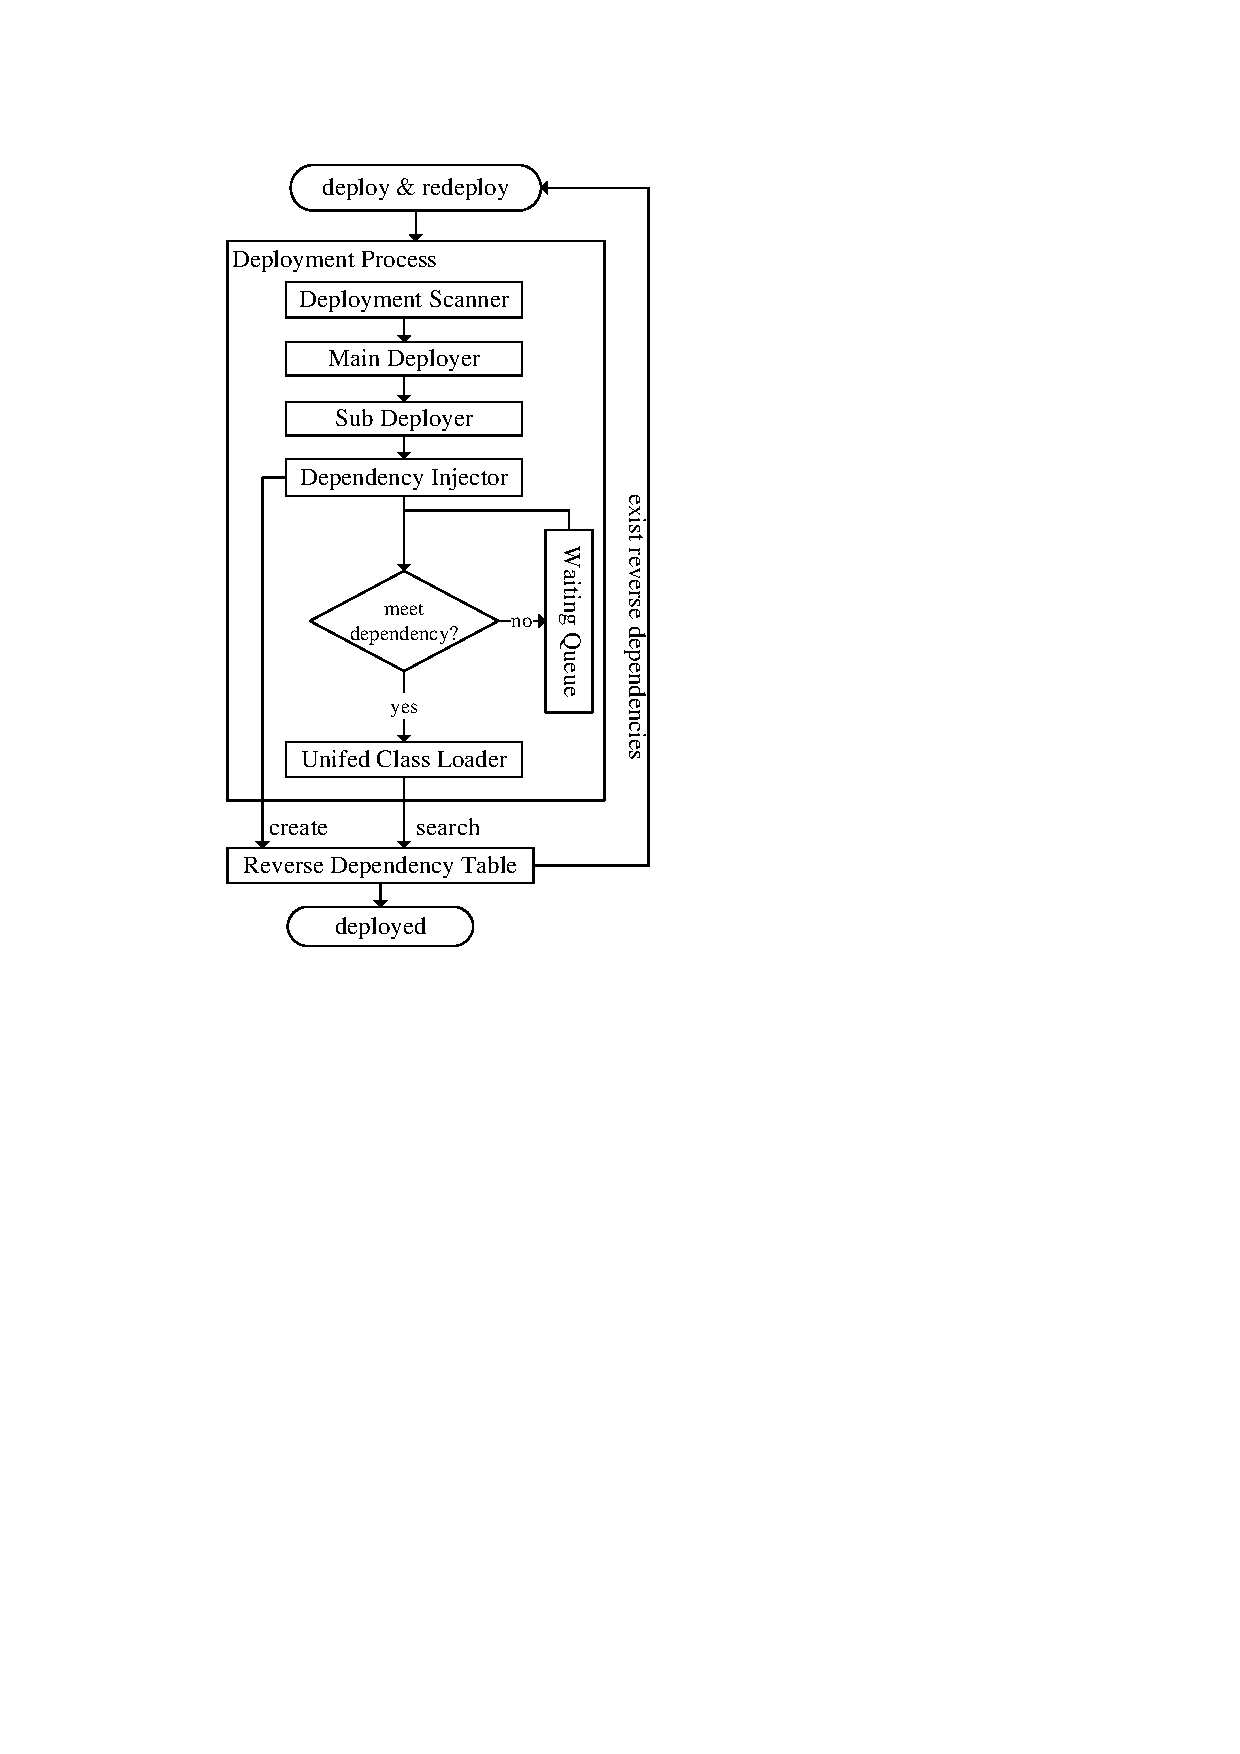
\includegraphics[width=2.2in]{ProcessReconstructionAS.pdf}
\caption{dependency reconstruction in application servers}
\label{fig:reconstruction_AS}
\end{figure}

Fig.\ref{fig:reconstruction_AS} is a logical block diagram of hot deployment with dependency reconstruction in application servers.
In order to reconstruct dependencies, if depended modules are redeployed the dependent modules must be redeployed too.  
We improve hot deployment capabilities and extend the deployment process by two steps. 
Firstly, a reverse dependency record is created in the reverse dependency mapping table, if an EJB module with dependency injection is deployed at the first time.
Secondly, when an EJB module is redeployed, we search the reverse dependency mapping table to find whether there are dependent modules depending on it and redeploy them at once if the reverse dependency exists.
In this semi-automatic way, we reconstruct dependencies simply and ensure the correctness of applications after hot deployment.

Although reconstruction in application servers can solve the problem of dependency loss and call failure, there are some disadvantages in the extension.
Not all the dependencies can be obtained from deployment process and be recorded in the reverse dependency mapping table.
Dependencies of inheritance or reference cannot be detected by dependency injector.
So application servers cannot reconstruct these kinds of dependencies and the problem of dependency loss still exists in most of modular applications.
In addition, this dependency reconstruction is a coarse granularity way to reconstruct and hot deploy modules.
All the dependent modules need to be redeployed, that means they will be handled through plenty of steps from the deployment process.
Actually, depended modules are the updated modules and updating dependent modules is just for reconstruct dependencies.
This causes application servers inefficient and also causes hot deployment inflexibility.

%// give the overview of the JBoss AS extension.
%// the deployment process, how to obtain dependencies
%// disadvantages
 
 
\section{Dependency Reconstruction in Class Loaders\label{sec:reconstructionCL}}

Application servers can manage dependencies of modules via the reverse dependency mapping table.
when hot deployment occurs, the reverse dependency mapping table helps application servers to search the dependent modules.
Dependencies of these modules are lost and they must be reconstructed.
However, these modules are still original versions.
Most of the work in redeploying dependent modules makes no sense except class loading in the modules.
Dependency management and reconstruction should be handled in the class loader.
Then dependent modules just need to reload the classes to reconstruct dependencies and most of the deployment process is omitted.
Updating efficiency is greatly improved.

Because each module has its own class loader, the dependencies of modules are just the dependencies of class loaders.
Each class loader that represents each module should record which class loaders it depends on.
At the same time, the class loader of the depended module should record what depends on itself as the reverse dependencies.
So, each class loader may have one or more depended class loaders and dependent class loaders.
All the information is collected when classes are loaded at the first time and their class loaders maintenance these important dependency information. 
From an overall perspective, these module class loaders constitute a dependency graph.
Every vertex of this graph can be regard as a class loader or a related module and every edge represents a dependency from one class loader to another.

The classes which are implemented by developers will be loaded by module class loader created in the deployment process, but the system classes, such as String, Object and so on, require system class loader or even bootstrap class loader to load them.
Parent delegation mechanism\cite{parent_delegation} ensures the safety and uniqueness of system classes.
This loading strategy gives priority to load class by parent class loader.
Bootstrap class loader has the highest priority and the next is extension class loader and system class loader.
The last is our module class loader which is defined by us.

Generally, there should be a parent class loader called system class loader in each module class loader.
This parent class loader can be treated as a depended class loader because the original class really depends on the system class which loaded by its parent class loader.
Based on parent delegation and our dependency graph for module class loaders, our class loader architecture model is organized in both a class loader hierarchy and a class loader network\cite{class_loader_patent}.

\begin{comment}
As we know, class loader is an important concept in Java projects and application servers based on J2EE\cite{j2ee}.
We implement to three safe and reliable module class loaders to support hot deployment of dependency reconstruction.
They are Circle Dependency Reconstruction Class Loader(CDR Class Loader) with static dependency management, Adaptive Dependency Reconstruction Class Loader(ADR Class Loader) and Adaptive Dependency Reconstruction Delay Class Loader(ADRD Class Loader) with dynamic dependency management.
Our customized class loaders not also complete basic class loading, but also maintain and reconstruct dependencies.
Thus, hot deployment and dependency reconstruction becomes more flexible and efficient.
\end{comment}

\subsection{Class Loader with Static Management}

Static dependency management is based on profiles of modules. 
The profile describes the module information including dependencies and main classes. 
It is named after the module in order to manage the module with a unified identification. 
For example, a profile named \emph{Compute.xml} in the module Compute.jar records the dependencies of Compute.jar. 
So dependency graph is created by profiles of all the modules. 
The dependent class loaders will be set in the class loader of each module.

\begin{algorithm}[ht]
\caption{function loadClass of \emph{Circle Class Loader}}
\label{alg:Circle_Class_Loader}
\begin{algorithmic}[1]
\REQUIRE ~~\\
Fully qualified name of the class: $name$ \\
Request time of class loading: $firstTime$

\ENSURE ~~\\
The loaded class instance: $c$

\STATE $c\leftarrow$\emph{findLoadedClass}($name$)

\IF {$c = null\ \&\&\ visitTime < firstTime$}

	\STATE $visitTime\leftarrow currentTime$
	
	\FOR {\textbf{each} class loader $dep$ in $depArrayList$}
		
		\STATE $c\leftarrow dep.$\emph{loadClass}($name$, $firstTime$)
		
		\IF {$c\ne null$}
			
			\STATE \textbf{return} $c$

		\ENDIF
	
	\ENDFOR

	\STATE $c\leftarrow$\emph{findClass}($name$)

\ELSE
	
	\STATE \textbf{return} $c$

\ENDIF


\end{algorithmic}
\end{algorithm}

We implement \emph{Circle Class Loader} with static dynamic management.
Algorithm \ref{alg:Circle_Class_Loader} shows \emph{Circle Class Loader} how to load classes. 
The class loader will try the dependent class loaders to load classes at first. 
We regard the system class loader as a dependent class loader of each module class loader to guarantee the safe loading of system classes. 
The dependency graph probably has a circle so that there must be a circle detection in the algorithm of loading classes. 
Under the definition of module dependency, class set $C$, class loader $L$ and dependencies $R$ of each module $M$ are determined from the dependency graph. 
Moreover, we can obtain the dependent class loader list of $L$ from each class loader of each module in $R$, which represents \emph{depArrayList} in Algorithm \ref{alg:Circle_Class_Loader}. 

If updating is detected, some affected class loaders and dependencies must be modified.
However, modifying the changing class loaders and their dependencies is not enough because dependencies may be lost while hot deploying depended modules.
For instance, if Validator.jar is updated, in order to reconstruct dependencies, all of modules which depend on Validator.jar also require to be updated even though they have no new versions and users don't want to update them.
So we reconstruct the dependencies for Validator.jar by updating these class loader of affected modules.
But reconstruction is not finished because these dependent modules may be depended on other modules.
We need to reconstruct their dependencies too in the same way, until there is no updated modules are depend on any of the updated modules.
All the affected modules should own their new class loader instance instead of the old one, because the old class loader has the cache of old classes and it cannot load the new classes with the same name.
Replacing the old class loaders is the most convenient way to update modules and reconstruct dependencies.
Meanwhile, updating the old class loader instances and dependencies is necessary.
In \emph{Circle Class Loader}, reconstruction process is similar to the process of creating dependency graph. 
The graph and \emph{Circle Class Loaders} are updated by the new version of profiles before the loading of classes. 
The dependencies are managed in \emph{Circle Class Loaders} based on the static profiles of modules.



\subsection{Class Loader with Dynamic Management}

\begin{figure*}[ht]
\centering
\subfloat[loading ComputeBean]
{
	\label{fig:subfig:a}
	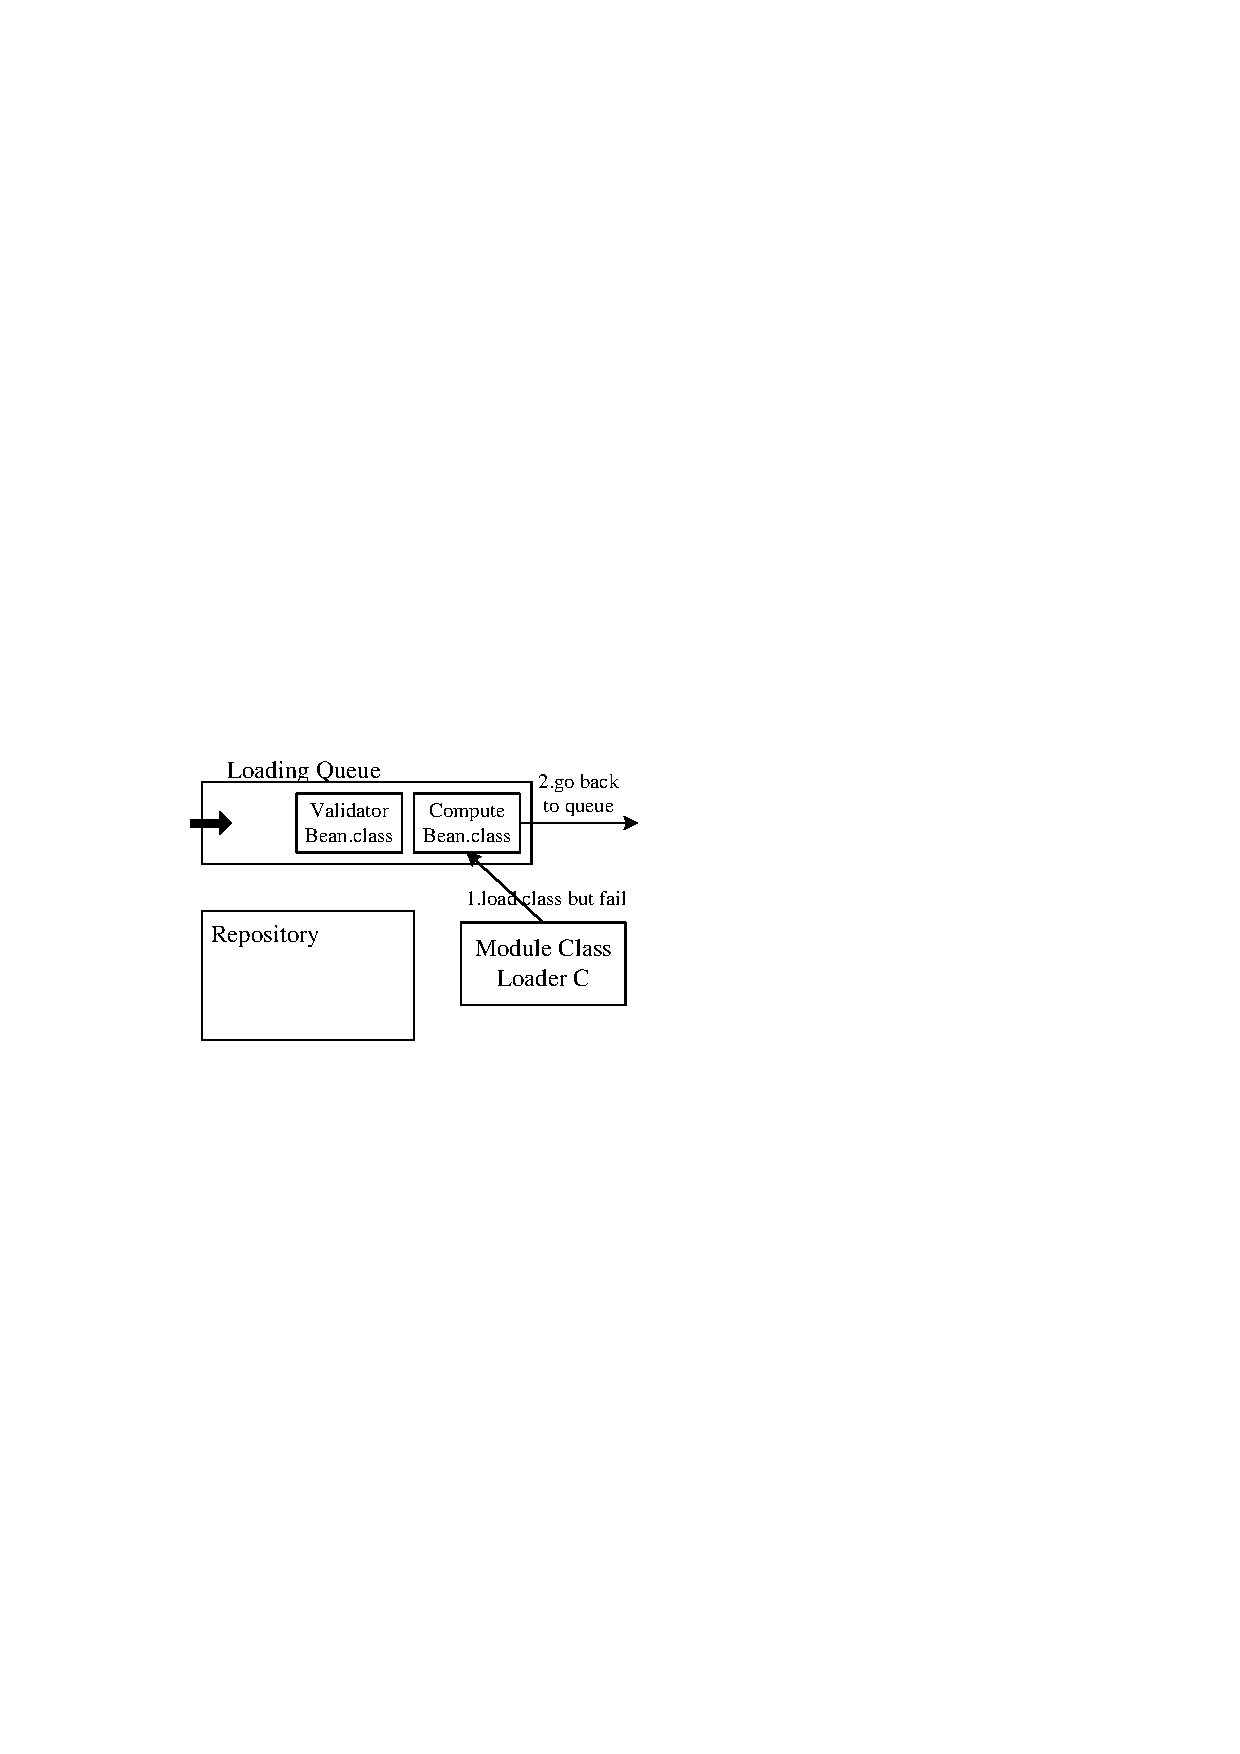
\includegraphics[height=1.4in]{LoadingQueueA.pdf}
}
\hfil
\subfloat[loading ValidatorBean]
{
	\label{fig:subfig:b}
	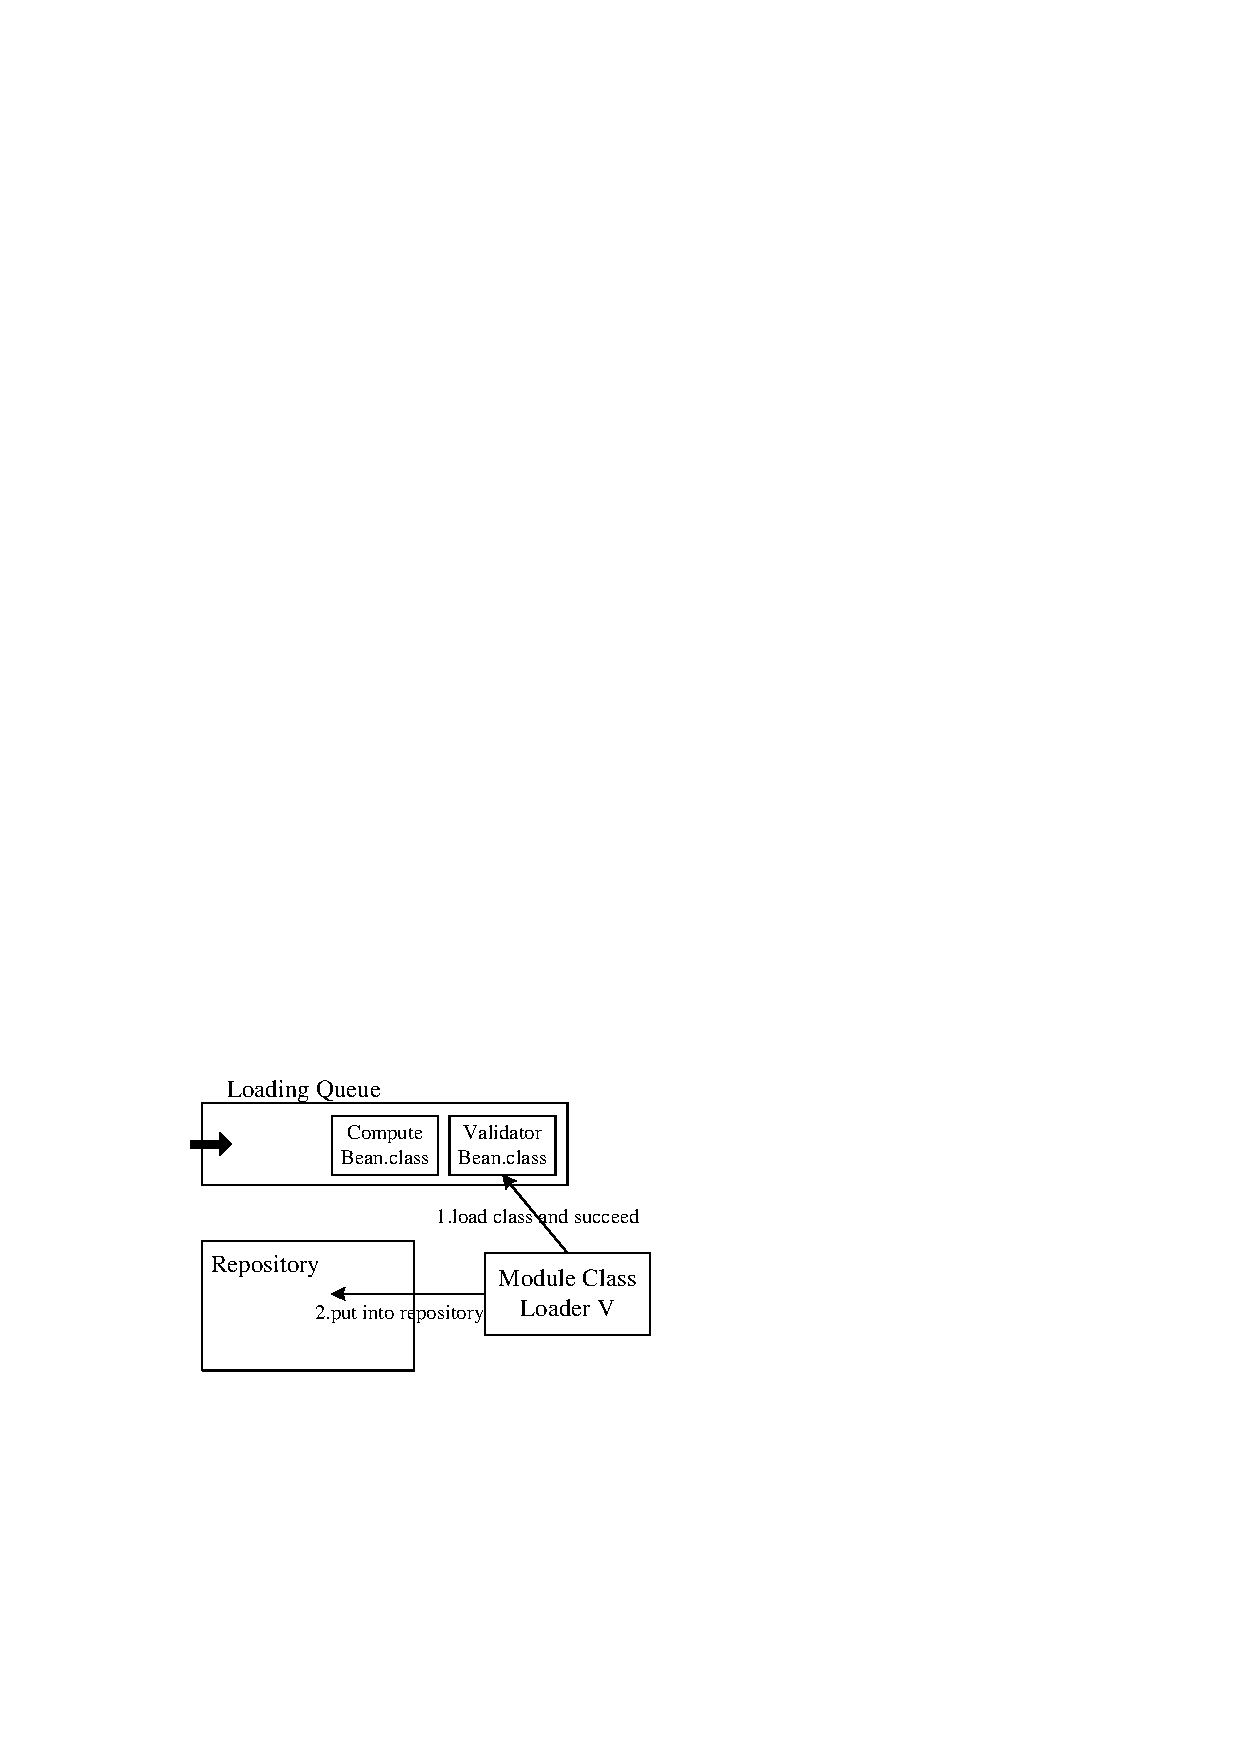
\includegraphics[height=1.4in]{LoadingQueueB.pdf}
}
\hfil
\subfloat[loading ComputeBean again]
{
	\label{fig:subfig:c}
	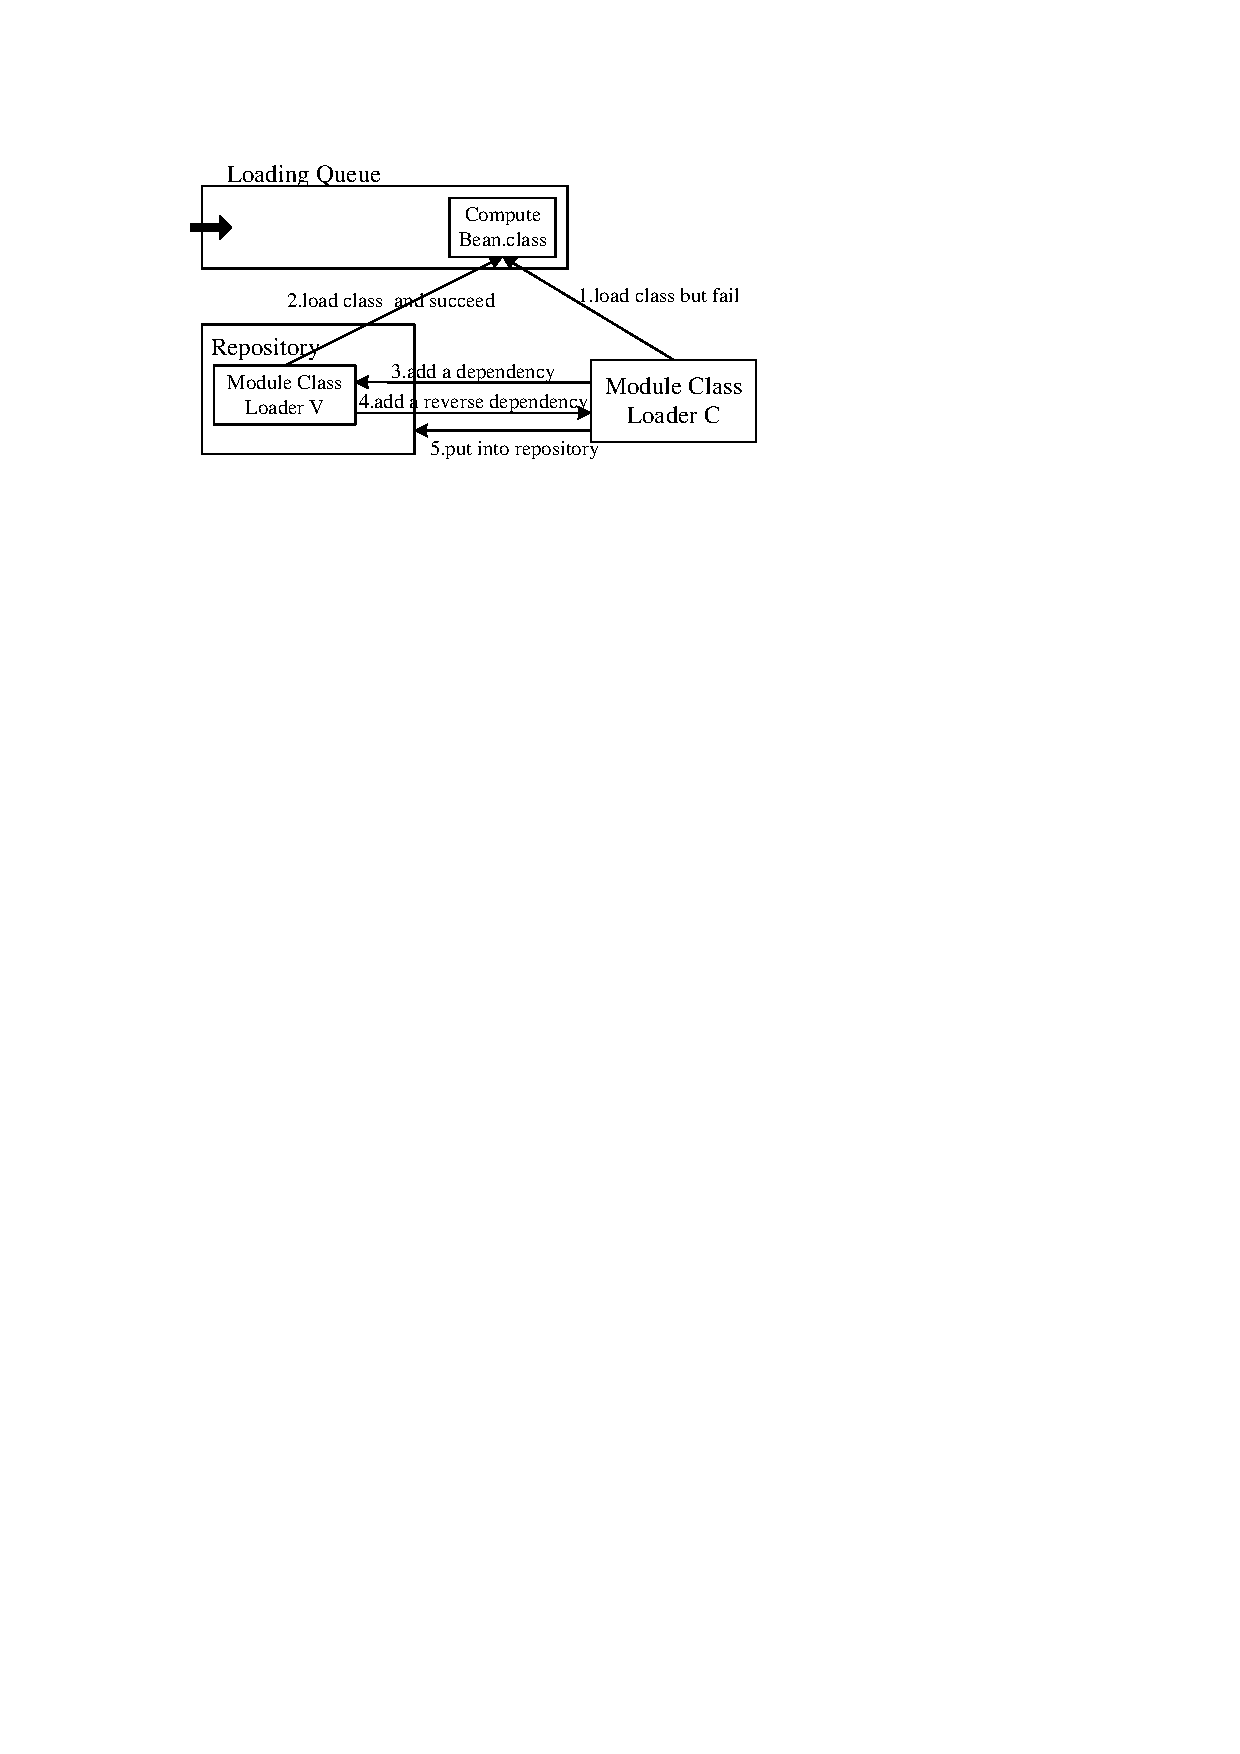
\includegraphics[height=1.4in]{LoadingQueueC.pdf}
}
\caption{details of loading classes via Adaptive Class Loader}
\label{fig:loading_queue}
\end{figure*}

Editing profiles of modules is a quite messy work when modular applications are composed of hundreds of modules.
Dynamic dependency management avoids this work because it has a loading queue to make a try when loading classes.
The loaded class will be placed in the repository and the unloaded class will enter the loading queue again to wait for the next loading.
Due to continuous trying, we can obtain dependencies of all the classes(modules) by an adaptive way.
The priority order of loading rules is described in the following:
\begin{itemize}[\IEEEsetlabelwidth{9}]
\item[1)] Try to use the system class loader to load it, if the class name begins with "java.".
\item[2)] Try to use its own class loader to load it.
\item[3)] Try to use its dependent class loaders to load it.
\item[4)] Try to use the class loaders which have already loaded other classes in the repository. 
\end{itemize}

Fig.\ref{fig:loading_queue} shows the loading classes process of the division EJB application that we used before. 
There are two classes \emph{ComputeBean} and \emph{ValidatorBean} in the application. 
We put them into the loading queue and try to load \emph{ComputeBean} at first. 
Due to the dependencies, module class loader $C$ which belongs to Compute.jar fails to load it. 
Class \emph{ComputeBean} should go back to the loading queue again to wait the next loading, which is described as Fig.\ref{fig:subfig:a}. 
Then it is turn to load Class \emph{ValidatorBean} in Fig.\ref{fig:subfig:b}. 
Module class loader $V$ loads it successfully, so we add the class loader into repository. 
With more classes loaded successfully, more class loaders will be put in the repository and they help to load other classes. 
Thus, \emph{ComputeBean} can be loaded successfully at the second time by the class loader in the repository as presented in Fig.\ref{fig:subfig:c}.
If a class loader in the repository loads the other class successfully, that means it is the dependent class loader of the other class loader and the dependency is created in the class loader incidentally. 
Finally, the loading queue becomes empty and all the classes are loaded with the dependencies.
Without static profiles, module class loaders create dependencies dynamically while loading classes, so we call this type of module class loader \emph{Adpative Class Loader}.

If hot deployment happens, the old version classes in the repository must be removed and their related dependencies must be dropped. 
Then, the new version classes are also placed in the loading queue and the process is just like deployment process. 
Dependency reconstruction in dynamic dependency management is similar with it in static dependency management. 
We can find out all the dependent modules group by group. 
No matter whether these modules have the new version, they must be removed in the repository as the old ones and then put them in the loading queue to be reloaded. 
So, all the lost dependences will be reconstructed by taking the place of the original class loaders and their dependent class loaders. 

\begin{figure}[ht]
\centering
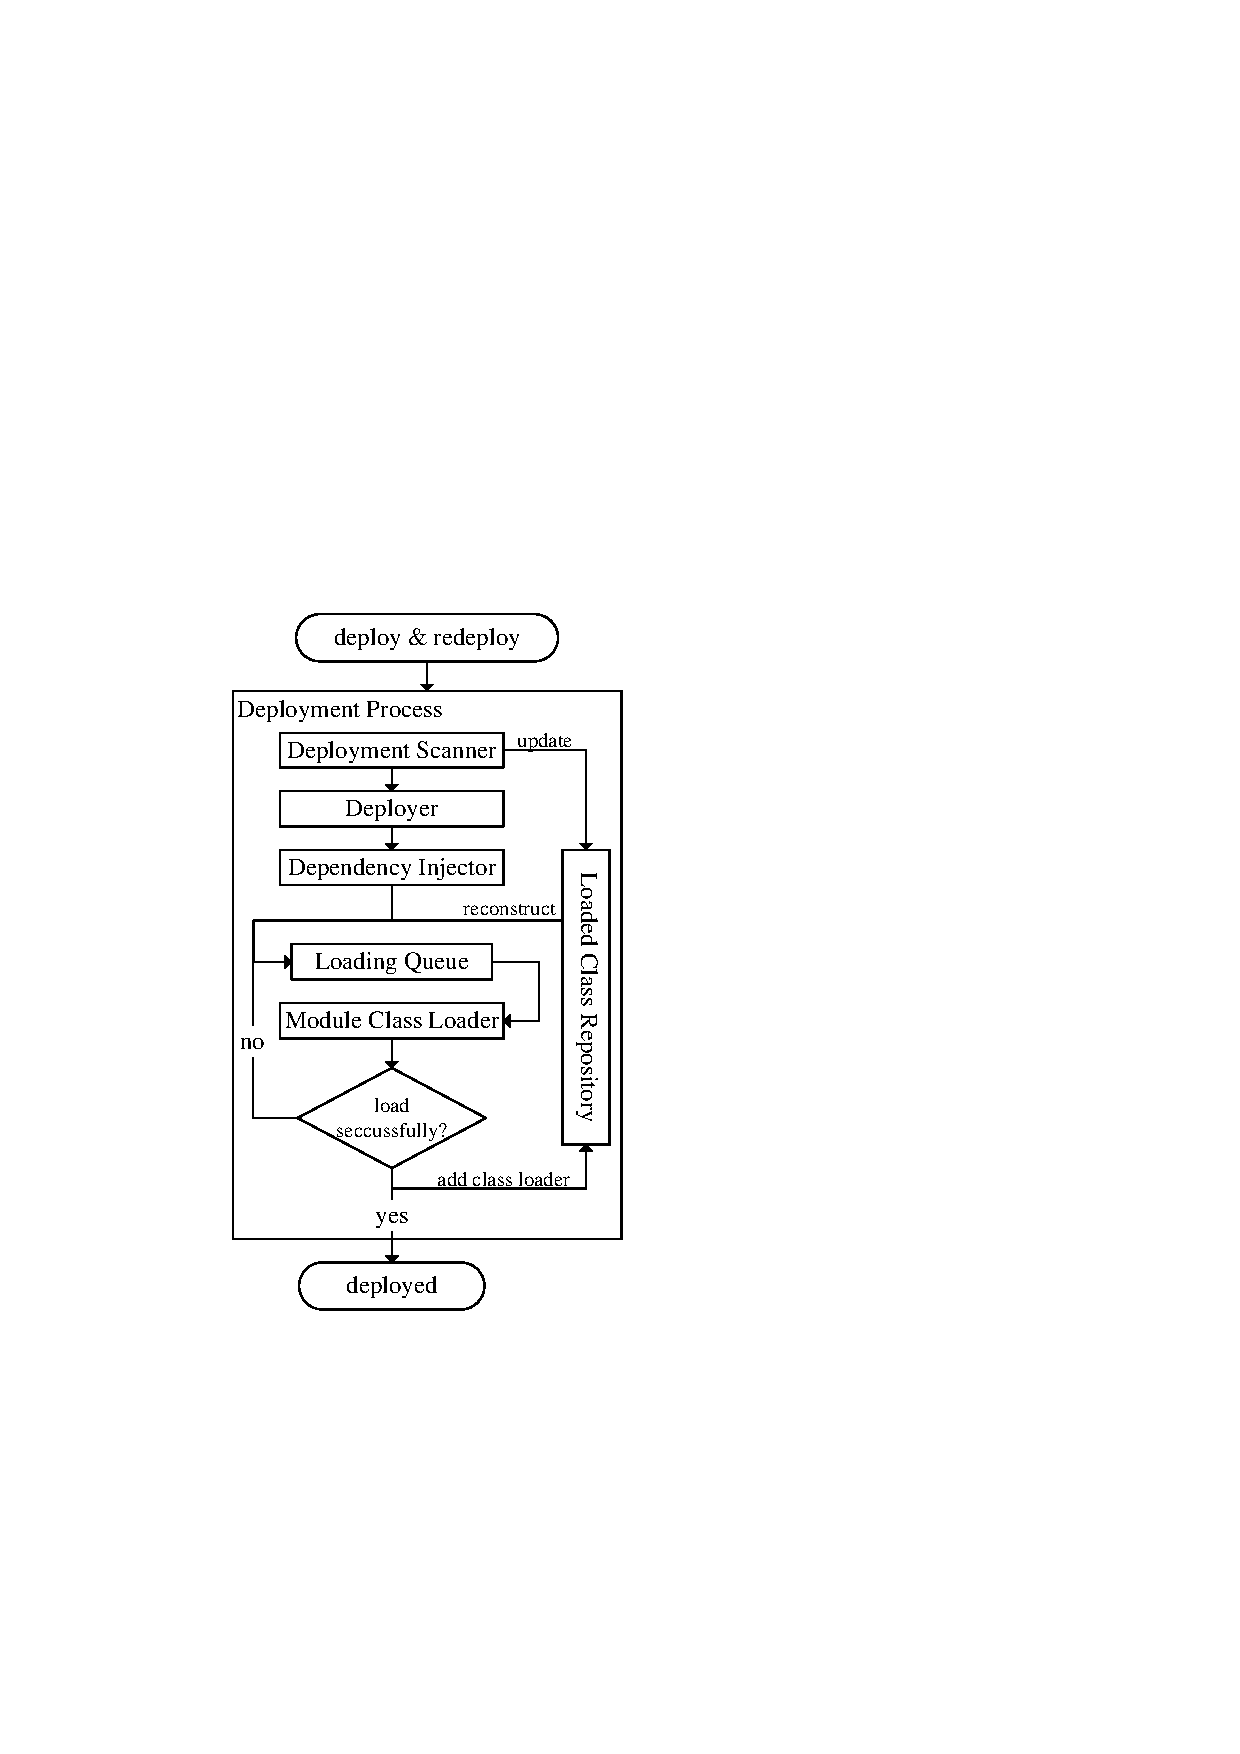
\includegraphics[width=2.2in]{ProcessReconstructionCL.pdf}
\caption{dependency reconstruction in class loaders}
\label{fig:reconstruction_CL}
\end{figure}

Fig.\ref{fig:reconstruction_CL} shows the whole process of hot deployment with dependency reconstruction in class loaders. 
The affected modules only update their module class loaders and the affected classes need to be reloaded through the loading queue, so that we save the part cost of redeployment process for the dependent modules which are still the old versions. 
Even though adaptive way to load class is time consuming, avoiding editing dependencies in the profiles of modules is a time saving thing for developers of modular applications or administrators of application servers.


\subsection{Class Loader with Lazy Reconstruction}

\begin{algorithm}[ht]
\caption{function loadClass of \emph{Delay Class Loader}}
\label{alg:Delay_Class_Loader}
\begin{algorithmic}[1]
\REQUIRE ~~\\
Fully qualified name of the class: $name$ \\

\ENSURE ~~\\
The loaded class instance: $c$

\STATE $c\leftarrow$\emph{findLoadedClass}($name$)

\IF {$c = null$}
	
	\IF {$name.$\emph{startWith}("java.")}
	
		\STATE $c\leftarrow systemClassLoader.$\emph{loadClass}($name$)
	
		\IF {$c \ne null$}

			\STATE \textbf{return} $c$
	
		\ENDIF

	\ELSE

		\STATE $c\leftarrow$\emph{findClass}($name$)

		\IF {$c = null$}

			\FOR {\textbf{each} class loader $dep$ in $depArrayList$}

				\STATE $c\leftarrow dep.$\emph{loadClass}($name$)

				\IF {$c\ne null$}
			
					\STATE \textbf{return} $c$

				\ENDIF
			
			\ENDFOR

			\FOR {\textbf{each} class loader $cl$ in $repository$}
				

				\IF {$cl.$\emph{valid} = false}

					\STATE $cl\leftarrow$\emph{reconstruct}($cl$)
				
					\STATE $cl.$\emph{valid}$\leftarrow$true

				\ENDIF

				\STATE $c\leftarrow cl.$\emph{loadClass}($name$)

				\IF {$c\ne null$}

					\STATE $depArrayList$.\emph{add}($cl$)
			
					\STATE \textbf{return} $c$

				\ENDIF
			
			\ENDFOR
	
	
		\ELSE

			\STATE \textbf{return} $c$

		\ENDIF

	\ENDIF

\ELSE

	\STATE \textbf{return} $c$

\ENDIF


\end{algorithmic}
\end{algorithm}

\emph{Delay Class Loader} is a type of module class loader with lazy reconstruction.
Comparing with \emph{Adaptive Class Loader}, \emph{Delay Class Loader} delays dependency reconstruction when hot deployment happens.
It is lazy for \emph{Delay Class Loader} to reconstruct dependencies at once. 
So all the affected class loaders only mark as invalid class loaders and none of class loaders are updated after hot deployment.
Dependency reconstruction will happen when applications are executed.
Because in this time, \emph{Delay Class Loaders} have to reconstruct dependencies to ensure the correctness of applications.
If the class loader is invalid, we should update and reconstruct it before using it to load classes. 
The algorithm of loading class is described in Algorithm \ref{alg:Delay_Class_Loader}, which uses the loading rules of \emph{Adaptive Class Loader}.
Similarly, dependency reconstruction process is also as the same as the reconstruction process of \emph{Adaptive Class Loader}.
Their main difference is their reconstruction time.
\emph{Delay Class Loader} reconstructs dependencies when applications are executed, so that it may save the time of hot deployment and avoid reconstruction if users never execute some modules after updating them.

\subsection{Contribution}
Our contribution is to propose a technology of hot deployment with dependency reconstruction.
From an engineering point of view, hot deployment with dependency reconstruction solves the problem of hot deploying modular applications in practical engineering projects.
Particularly, we customize the class loader which can manage dependencies of modules.
Then we can reconstruct dependencies in the class loader, so that we improve the efficiency of hot deployment.
In the future, we can split a module into several sub modules or assemble some sub modules of different modules according their original dependencies.
Each class loader only the loads classes of corresponding sub modules.
So reconstruction in class loaders reduces the granularity of the update and narrows the scope of the hot deployment.
The hot deployment becomes more flexible. 

%// how to reconstruct, (we can find the dependencies in the class loader)
%// why updating class loaders is neccessary
%// our contribution


\section{Evaluation\label{sec:evaluation}}
In this section, we did some evaluations on efficiency, dynamic feature and flexibility for our technology of hot deployment with dependency reconstruction.

\subsection{Experiment}
Mainstream application servers only support hot deployment of standalone applications, which cannot satisfy the requirement of modular applications.
Hot deployment with dependency reconstruction can ensure the correctness of the modular applications.
We use a simple division modular application in Fig.\ref{fig:example} to evaluate the hot deployment with dependency reconstruction.
And our experimental environment is following:
\begin{itemize}[\IEEEsetlabelwidth{9}]
\item[1)] OS: Ubuntu 12.04
\item[2)] JDK: Java Version "1.6.0\_24"
\item[3)] IDE: Eclipse IDE for Java EE Developers
\item[4)] AS: JBoss AS 5.1.0 \& JBoss AS 5.1.0 extension(Reconstruction in AS)
\end{itemize}

We start the application server and deploy two session beans called Compute.jar and Validator.jar and we can compute division correctly through this modular application.
Then we only update Validator.jar.
After hot deployment, the application in JBoss AS 5.1.0 will throw the EJB exception when we use Compute.jar to do division of two numbers.
However, JBoss AS 5.1.0 extension reconstructs lost dependencies and redeploys Compute.jar, so that we can make the calculation without exception.
Dependency reconstruction guarantees the correctness of hot deploying dependent modules in modular applications.

\subsection{Efficiency}


\begin{table*}
\centering
\caption{time cost of redeployment}
\label{tab:stage}
\begin{tabular}{|c|c|c|c|c|}
\hline
\emph{Module Name}	&	\emph{Configuration Stage}	&	\emph{Distribution Stage}	&	\emph{Total Time}	&	\emph{Promotion Rate}\\
\hline
\hline
Compute.jar		&	13ms			&	33ms			&	46ms			&	28.3\%\\
\hline
Validator.jar		&	12ms			&	29ms			&	41ms			&	29.3\%\\
\hline
pestore.jar(1.1.2)	&	34ms			&	236ms			&	270ms			&	12.6\%\\
\hline
pestore.jar(1.3.2)	&	24ms			&	113ms			&	137ms			&	17.5\%\\
\hline
netboot.war		&	19ms		 	&	65ms			&	84ms			&	22.6\%\\
\hline
persistent-service.sar 	& 	14ms 			&	35ms			&	49ms			&	28.6\%\\
\hline
ejb-management.jar	& 	12ms		 	&	283ms			&	295ms			&	4.1\%\\
\hline
derby-plugin.jar	&	16ms			&	16ms			&	32ms			&	50.0\%\\
\hline
threaddump.war		&	10ms			&	52ms			&	62ms			&	16.1\%\\
\hline
jbossts-tools.sar	&	21ms			&	87ms			&	108ms			&	19.4\%\\
\hline
jbossxts.sar		&	52ms			&	860ms			&	912ms			&	5.7\%\\
\hline
\end{tabular}
\end{table*}

Comparing with JBoss AS 5.1.0, the application server extension, using dependency reconstruction in application servers, needs more time to hot deploy modules because the server searches dependencies in the reverse dependency table and deploys more dependent modules.
But this type of dependency reconstruction can guarantee the correctness of hot deployment without restarting application servers.
Obviously, the hot deployment with dependency reconstruction which can avoid restarting servers is more efficient.

Reconstruction in application servers is a native way to solve the call failures because many dependent modules of original versions are redeployed after the depended modules.
However, most of the work in redeploying dependent modules makes no sense except class loading in the modules.
Reconstruction in class loaders improves updating efficiency because dependency management and reconstruction is handled in the class loader most of the deployment process is omitted.

According to deployment specification\cite{jsr88}, deployment is typically a three-stage process: configuration, distribution and start execution.
We focus on the first two stages in our experiments.
Deployment context of modules are creatd in configuration stage, but they are not changed when redeployment of dependent modules happens.
We use the original context and only update its module class loader before distribution stage which is responsible for installing modules and loading classes.
So we save the time used to create and set the deployment context in the redeployment process.

Table \ref{tab:stage} shows the cost of redeployment in these two stages for some modules and applications.
Compute.jar and Validator.jar are two session beans which constitute an example application of division in Fig. \ref{fig:example}.
Java Pet Store\cite{java_pet_store} is a sample well-known application from the J2EE\cite{j2ee}, so it is also one of our subjects.
The rest testing modules are services of JBoss, which can be found in the examples directory of JBossAS 5.1.0 Release.
We hot deploy them when the application server is running and calculate the time cost of the configuration stage and distribution stage.
In our approach of reconstruction in class loaders, the time cost of the configuration stage will be saved when hot deployment happens.
Moreover, dependent modules won't update themselves in the deployment directory and the scanning time, which is 5 seconds as default configuration, is saved and that means applications don't require to wait for the class loading delay of dependent modules. 
The efficiency is highly improved according to the promotion rate of Table \ref{tab:stage}.

\subsection{Dynamic Feature}
Comparing with \emph{Circle Class Loader} based on static dependency management, \emph{Adaptive Class Loader} and \emph{Delay Class Loader} can obtain the dependencies of modules in the dynamic way.
By several trying, we can create the dependency graph on the basis of whether the class is loaded successfully.
Developers don't configure the profile of modules to describe the dependencies of the modules.
The dependencies are managed and reconstructed dynamically at any time.

Actually, static dependency management is more efficient than dynamic dependency management in terms of deployment and redeployment time.
Distribution stage accounts for a large proportion of the total deployment process according to Table \ref{tab:stage}.
\emph{Adaptive Class Loader} and \emph{Delay Class Loader} may try to load a class for many times if this class depends on other classes which are packaged in different modules.

However, the advantage of dynamic feature is reducing management of modules for developers.
As we know, enterprise applications probably contain hundreds of modules and complex dependencies.
It is annoying for developers to create and manage configuration files of each module if there are no reliable automatic tools for generating them.
Additionally, dynamic feature makes hot deployment more flexible, which we will talk about in the following part.


\subsection{Flexibility}

\begin{table*}
\centering
\caption{performance of flexibile reconstruction}
\label{tab:flexibility}
\begin{tabular}{|c|c|c|c|c|}
\hline
\emph{Loading Strategy}	& \emph{Deploy and Execute All}	& \emph{Redeploy and Execute All} & \emph{Redeploy and Execute One}\\
\hline
\hline
Adative Class Loader 	&	94ms				&	142ms				&	52ms\\
\hline
Delay Class Loader 	&	92ms				&	137ms				&	43ms\\
\hline
\end{tabular}
\end{table*}

\begin{figure}[ht]
\centering
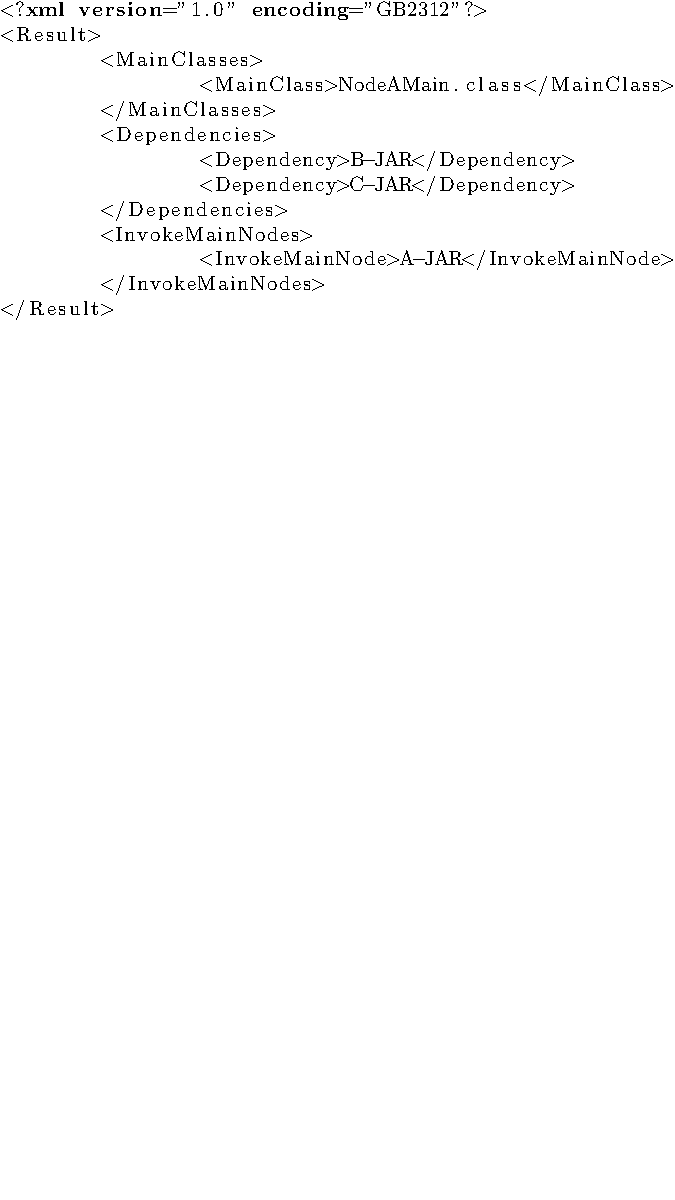
\includegraphics[width=3.5in]{xmlpicture.pdf}
\caption{A-JAR.xml file}
\label{fig:xml_pic}
\end{figure}

The class loader is an important part in application servers based on J2EE.
Reconstruction in class loaders make hot deployment more flexible.
On the one hand, dynamic dependency management allows class loaders to construct dependencies in the attempt to load classes without configuration files.
On the other hand, reconstruction can be carried out at any time before execution of applications.
The dependency reconstruction of \emph{Adaptive Class Loader} is in the process of hot deployment, which means the class loaders finish reconstructing dependencies when the application servers complete hot deployment.
In contrast, \emph{Delay Class Loader} which should be reconstructed is marked as invalid when hot deployment happens.
The class loaders and their dependencies won't be updated until the applications start to be executed.
So, we handle invalid class loaders and reconstruct them at the time of application execution.
Comparing with \emph{Adaptive Class Loader}, \emph{Delay Class Loader} delays reconstruction and increase the flexibility of reconstruction.

In a particular application scenario, \emph{Delay Class Loader} Class Loader has a good performance. 
We compare performance of flexible reconstruction between \emph{Adaptive Class Loader} and \emph{Delay Class Loader} through experiments.
We choose a simple modular application with three modules A, B and C.
Module A depends on Module B and C, which is described as profile of Module A in Fig.\ref{fig:xml_pic}.
Then we copy this application for 20 times and build 20 modular applications with identification from 1 to 20.
In the experiment, we deploy 20 applications with 60 modules in the application servers and execute all of them.
Then we hot deploy Module B of all the applications.
To ensure the correctness of applications, module A and B need to be reconstructed.
After redeployment, we execute all the applications so that all of class loaders finish reconstructing.
If we execute only one of applications, only \emph{Delay Class Loader} of this application modules will complete reconstruction.
So, the time of hot deployment and execution decreases in Table \ref{tab:flexibility}. 



\section{Related work\label{sec:relatedwork}}

The concept of modularity was proposed a long time ago by Divid Parnas\cite{Divid_specification}.
He gave two main criteria\cite{Divid_criteria} to be used in decomposing systems into modules in 1972.
They were making each major step in the processing module and using information hiding as a criterion.
After that, people gradually changed the way of developing software.
And Modularity impacts on development, deployment, operation, maintenance in software engineering until now.
So, many researchers focus on modularity and modular applications in all fields of software engineering, such as software metric\cite{module_metric} and software testing\cite{module_test}.
Even some new technologies and concepts(e.g. AOP\cite{module_aop} and cloud\cite{module_cloud}) of software engineering also have related to modularity and modular applications.

Although many researchers dedicated to the study of hot deployment, most of the work focused on the hot deployment of distributed heterogeneous environments\cite{related_hot_1, related_hot_2, related_hot_3, related_hot_4}.
They solved problems about the dynamic service creation, service life cycle management and other issues based on OGSA (Open Grid Service Architecture).
In terms of dependency injection, most of the work focused on the dependency injection mechanism and its performance in different environments\cite{related_DI_1, related_DI_2, related_DI_3}.
They involved a number of fields, such as distributed applications, design patterns, and software maintenance.
In contrast, our work proposes a technology of hot deployment with dependency reconstruction, which makes hot deployment more flexible and efficient.

Improving abilities of application servers through component extension is not a new idea.
For example, Li et al. advocated an on demand approach of deploying services in application servers\cite{related_AS_1} and they even proposed an approach to make an application server well-structured and dynamic\cite{related_AS_2}.
And some research focused on refactoring application servers according to application requirements\cite{related_AS_3}.
	
On the other hand, application servers can preprocess modules before modular applications are deployed.
It brings many benefits in performance. For instance, several modules merge into one module to reduce dependencies\cite{related_merge} or a module splits into several ones in order to reduce the cost of update\cite{related_split}.
It is also helpful to our future work on dependency reconstruction in class loaders.
In this way, we will decrease the granularity of update and reconstruction.


\section{Conclusion and future work\label{sec:conclusion}}
Hot deployment mechanism is one of the typical features of mainstream application servers.
However, mainstream application servers cannot meet the demand with hot deployment of modular applications.
This paper proposes a technology of hot deployment with dependency reconstruction.
In order to make hot deployment becomes more flexible and efficient, dependency reconstruction is implemented by several ways, including static profiles way, adaptive loading way and dynamic management with lazy reconstruction.
Experiment shows the problem of calling failure can be solved through this technology and the efficiency of application servers is improved.

In future, we will focus on reconstruction in class loaders.
Managing dependencies in class loaders make it possible to decrease the granularity of update and reconstruction.
Due to the more flexible hot deployment, the efficiency of application servers will be highly increased.
Moreover, we will implement dependency reconstruction in the code level\cite{future_Gu}, so that code-level dynamic update will be achieved and it will continue to decrease the granularity of update.


% conference papers do not normally have an appendix
% use section* for acknowledgement
\section*{Acknowledgment}
This work was supported in part by National Basic Research 973 Program(Grant No. 2015CB352202), and National Natural Science Foundation(Grant Nos. 61472177, 91318301, 61321491, 61361120097) of China.

% may modify acknowledgment



% references section
\begin{thebibliography}{9}

\bibitem{app_server}
What is an App Server, \url{http://www.theserverside.com/news/1363671/What-is-an-App-Server}.

\bibitem{jboss}
JBoss Application Server, \url{http://www.jboss.org}.

\bibitem{weblogic}
Oracle WebLogic Server, \url{http://www.oracle.com/technetwork/middleware/weblogic/overview/index.html}.

\bibitem{middleware_reliability}
Huang, Gang, et al. "Simulation-based analysis of middleware service impact on system reliability: Experiment on Java application server." Journal of Systems and Software 84.7 (2011): 1160-1170.

\bibitem{standard_cl}
Taylor, B. "Java Class Loading: The Basics." (2003).

\bibitem{module_cl}
Gangadharan, Binod Pankajakshy, Srikanth Padakandla, and Sivakumar Melapannai Thyagarajan. "Hot deployment of shared modules in an application server." U.S. Patent No. 7,721,277. 18 May 2010.

\bibitem{jboss_class_loader}
The JBoss JMX Microkernel, \url{http://docs.jboss.org/jbossas/jboss4guide/r5/html/ch2.chapter.html}.

\bibitem{DI}
Fowler, Martin. "Inversion of control containers and the dependency injection pattern." (2004).

\bibitem{EJB}
JSR 220: Enterprise JavaBeans\textsuperscript{\texttrademark} 3.0, \url{https://www.jcp.org/en/jsr/detail?id=220}.


\bibitem{jvm}
Java Virtual Machine, \url{http://java-virtual-machine.net/sun-java-virtual-machine.html}.

\bibitem{jvm_book}
Zhiming, Zhou. "Understanding the JVM Advanced Features and Best Practices." (2011).

\bibitem{jvm_specification}
The Java Virtual Machine Specification, \url{http://docs.oracle.com/javase/specs/jvms/se7/html}.

\bibitem{deployment_process}
Olliges, Sascha. Runtime Reconfiguration in J2EE Systems. Diss. Master Thesis supervised by Jasminka Matevska and Wilhelm Hasselbring, University of Oldenburg, Germany, Department of Computing Science, Software Engineering Group, 2005.

\bibitem{parent_delegation}
Rohit Chaudhri. "Understnding the Java Classloading Mechanism." Java Developer's Journal Vol.8, Issue 8, p.16.

\bibitem{class_loader_patent}
Meduri, Subbarao K., Thomas Edward Musta, and James Lee Van Oosten. "Collaborative classloader system and method." U.S. Patent No. 7,870,546. 11 Jan. 2011.

\bibitem{jsr88}
JSR-000088, Deployment API Specification, \url{http://jcp.org/aboutJava/communityprocess/mrel/jsr088/index.html}.

\bibitem{java_pet_store}
Java Pet Store, \url{http://www.oracle.com/technetwork/java/petstore1-3-1-02-139690.html}.

\bibitem{j2ee}
Bodoff, Stephanie, ed. The J2EE tutorial. Addison-Wesley Professional, 2002.



\bibitem{Divid_specification}
Parnas, David Lorge. "A technique for software module specification with examples." Communications of the ACM 15.5 (1972): 330-336.

\bibitem{Divid_criteria}
Parnas, David Lorge. "On the criteria to be used in decomposing systems into modules." Communications of the ACM 15.12 (1972): 1053-1058.

\bibitem{module_metric}
Kazemi, Ali, et al. "A metric suite for measuring service modularity." Computer Science and Software Engineering (CSSE), 2011 CSI International Symposium on. IEEE, 2011.

\bibitem{module_test}
Judge, Lyndon, et al. "A modular testing environment for implementation attacks." BioMedical Computing (BioMedCom), 2012 ASE/IEEE International Conference on. IEEE, 2012.

\bibitem{module_aop}
Przybyłek, Adam. "Where the truth lies: AOP and its impact on software modularity." Fundamental Approaches to Software Engineering. Springer Berlin Heidelberg, 2011. 447-461.

\bibitem{module_cloud}
Wettinger, Johannes, et al. "Enabling Dynamic Deployment of Cloud Applications Using a Modular and Extensible PaaS Environment." Cloud Computing (CLOUD), 2013 IEEE Sixth International Conference on. IEEE, 2013.

\bibitem{related_hot_1}
Florian, Vladimir, Gabriel Neagu, and Stefan Preda. "An OGSA Compliant Environment for eScience Service Management." P2P, Parallel, Grid, Cloud and Internet Computing (3PGCIC), 2010 International Conference on. IEEE, 2010.

\bibitem{related_hot_2}
Dornemann, Kay, and Bernd Freisleben. "Discovering Grid Resources and Deploying Grid Services Using Peer-to-Peer Technologies." Advanced Information Networking and Applications Workshops, 2009. WAINA'09. International Conference on. IEEE, 2009.

\bibitem{related_hot_3}
Friese, Thomas, Matthew Smith, and Bernd Freisleben. "Hot service deployment in an ad hoc grid environment." Proceedings of the 2nd international conference on Service oriented computing. ACM, 2004.

\bibitem{related_hot_4}
Abdellatif, Takoua, Jakub Kornas, and J-B. Stefani. "Reengineering J2EE servers for automated management in distributed environments." Distributed Systems Online, IEEE 8.11 (2007): 1-1.

\bibitem{related_DI_1}
Heinrich, Matthias, et al. "Enriching web applications with collaboration support using dependency injection." Web Engineering. Springer Berlin Heidelberg, 2012. 473-476.

\bibitem{related_DI_2}
Rajam, Sidhant, et al. "Enterprise service bus dependency injection on mvc design patterns." TENCON 2010-2010 IEEE Region 10 Conference. IEEE, 2010.

\bibitem{related_DI_3}
Razina, Ekaterina, and David S. Janzen. "Effects of dependency injection on maintainability." Proceedings of the 11th IASTED International Conference on Software Engineering and Applications: Cambridge, MA. 2007.

\bibitem{related_AS_1}
Li, Yan, et al. "Enabling on demand deployment of middleware services in componentized middleware." Component-Based Software Engineering. Springer Berlin Heidelberg, 2010. 113-129.

\bibitem{related_AS_2}
You, Chao, et al. "Towards a well structured and dynamic application server."Computer Software and Applications Conference, 2009. COMPSAC'09. 33rd Annual IEEE International. Vol. 1. IEEE, 2009.

\bibitem{related_AS_3}
Zhang, Charles, Dapeng Gao, and Hans-Arno Jacobsen. "Towards just-in-time middleware architectures." Proceedings of the 4th international conference on Aspect-oriented software development. ACM, 2005.

\bibitem{related_merge}
Brannen, Samuel Hugh, et al. "Computer system and a method of deploying an application in a computer system." U.S. Patent No. 8,359,590. 22 Jan. 2013.

\bibitem{related_split}
Sánchez, Iván Bernabé, Daniel Díaz-Sánchez, and Mario Muñoz-Organero. "Optimizing OSGi Services on Gateways." Ambient Intelligence-Software and Applications. Springer International Publishing, 2013. 155-162.

\bibitem{future_Gu}
Gu, Tianxiao, et al. "Javelus: A Low Disruptive Approach to Dynamic Software Updates." Software Engineering Conference (APSEC), 2012 19th Asia-Pacific. Vol. 1. IEEE, 2012.

\end{thebibliography}


% that's all folks
\end{document}


